
% \nb{Attempt at iteratively building up an explanation of proposed data provenance capture solution}

%\subsection{Data Provenance Capture}
\subsection{Computational Pipelines that Capture Provenance}

% data as node or edge?
For human interpretation, data processing workflows are commonly represented as a flowchart showing the data inputs, processes that operate on them, and final outputs of the system. For purposes of workflow automation (i.e. allowing machines to automatically execute the workflow) the data processing flowcharts are typically formalised as a graph (also known as a network) data-structure \cite{Bowers2006, Wu2016}. Nodes (also known as vertices) are used to represent inputs and processes, and edges (also known as arcs) are used to represent the flow of data between each process. The edges are directed to represent the direction of data flow (the input dependencies of a processes are in the reverse direction to the data flow). Under the assumption that there are no cyclic dependencies (i.e. an output that (indirectly) depends on itself), the graph is said to be a \textit{Directed Acyclic Graph} (DAG). An example workflow (pipeline) for computing a sport player's goal accuracy is provided in \figref{fig:simple-chain}.

%(image of a DAG for a simple pipeline)
%(similarity to flow charts / data flow diagrams)
%(formalise as a data flow diagram so that we have both data and processes)

\begin{figure}[h]
\centering
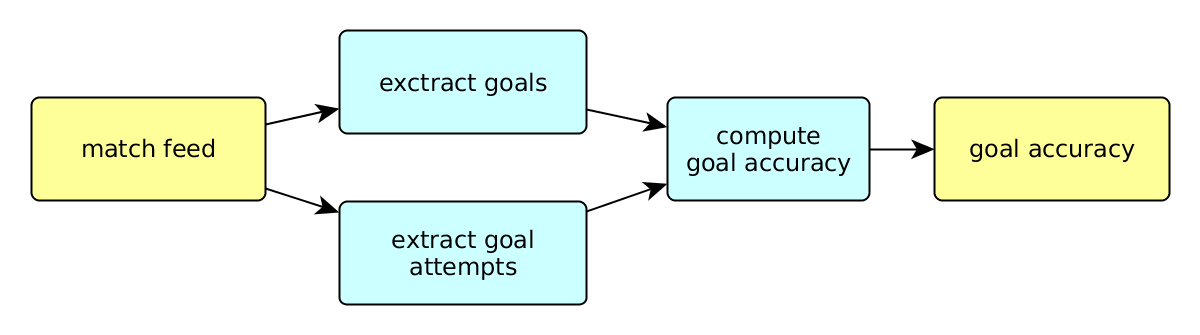
\includegraphics[width=\linewidth]{figs/dag/simple-dag-no-interpediates.png}
\caption{Example of a simple data processing workflow flowchart (formally, a directed acylcic graph)}
\label{fig:simple-chain}
\end{figure}

Optionally, additional nodes can be introduced to represent the intermediate data output of each process. Under this representation, there are two types of nodes: data nodes and process nodes, with chains that alternate data, process, data, process, etc. While this form is more cumbersome to write, it can help with formalisation. This is similar to the notation used by \textit{Data Flow Diagrams} (DFDs). An example pipeline marking these intermediate data outputs is shown in \figref{fig:simple-chain-intermediate}.

% \todo{Compare to UML activity diagrams, Business process modelling notation, Petri nets}

\begin{figure}[h]
\centering
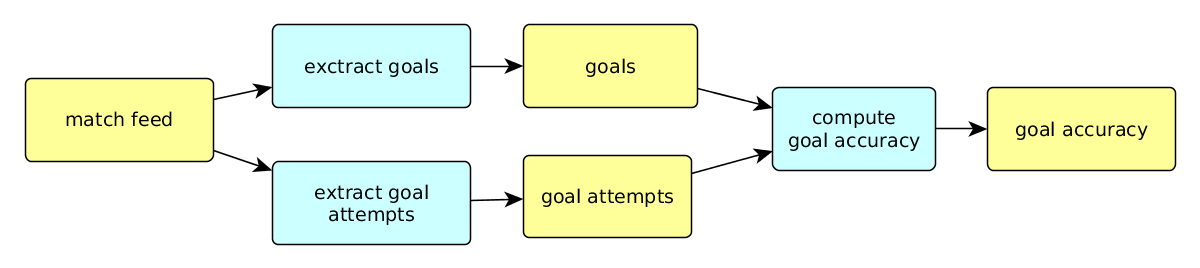
\includegraphics[width=\linewidth]{figs/dag/simple-dag.png}
\caption{Example of a simple data processing workflow with intermediate outputs explicitly shown}
\label{fig:simple-chain-intermediate}
\end{figure}

% (Image of DFD for pipeline)

While such pipelines are sufficient for describing processes, or in some cases automating them, it is also necessary to consider the description of the processes themselves. Assuming the process can be precisely described as written software (as opposed to a task that a human performs), then there is a need to track the version of the software used, as well as the environment that it requires. While in principle, software source code should unambiguously describe the actions it performs, in practice source code may have complex dependencies and assumptions about the environment that need to be met in order to build it into an executable. As the provenance of data depends critically upon the processes that are applied to it, capturing the provenance of the software is a prerequisite for capturing the full provenance of the data. In the software engineering community, the ability to reproduce the generated executable byte-for-byte from the software source code is known as a ``reproducible build''. While many mainstream software packages do not offer reproducible builds\footnote{E.g. the GNU/Linux Operating System distribution Debian notes that ``Reproducible builds of Debian as a whole is still not a reality''. \url{https://wiki.debian.org/ReproducibleBuilds}. Accessed: \dt{2019-01-19}}, certain security focused software such as the IP anonymisation network Tor and the encrypted messaging app Signal\footnote{Blog: Signal, 2016, ``Reproducible Signal builds for Android''. \url{https://signal.org/blog/reproducible-android/}} offer fully reproducible builds\footnote{A short history of open source software supporting reproducible builds is maintained by Wikipedia Contributors, ``Reproducible builds''. \url{https://en.wikipedia.org/wiki/Reproducible_builds} Accessed: \dt{2019-01-16}}.

However, reproducible builds only concern themselves with deriving software from source code. It is left to the user to manage provision of inputs and outputs to the resultant software artefact. Note however, that code and data are equivalent. A Turing machine, a mathematical model for describing computations, takes data on a (theoretically infinite) tape as its input, but can also be used to execute or manipulate a program on the tape as if it were data. Similarly, inputs that are supposedly data, may actually function as code\footnote{For example, the blog ``Accidentally Turing-Complete'' contains a list of data processing systems (such as templating engines) that have been proven Turing Complete despite never having been intended as programming languages. \url{http://beza1e1.tuxen.de/articles/accidentally_turing_complete.html} Accessed: \dt{2019-01-16}}, a fact that malicious users often take advantage of in order to execute arbitrary computations.

Development of reproducible build tools has focused of code transformations while ignoring the user supplied data inputs and outputs of the resultant program. In contrast, development of data provenance frameworks has focused on the flow of data inputs through data processing pipelines with little attention to capturing the provenance of the software itself that makes up the pipelines. However, the equivalence of code and data means that reproducible builds and data provenance capture are equivalent problems which can be unified into a single framework. A simple example to demonstrate the equivalence of data provenance capture to reproducible builds, is presented in \figref{fig:simple-chain-cmp}.


% Not a contribution
% \todo{Highlight unification of reproducible builds and data provenance frameworks as a contribution (and search literature for any prior work)}


\begin{figure}[h!]
\centering
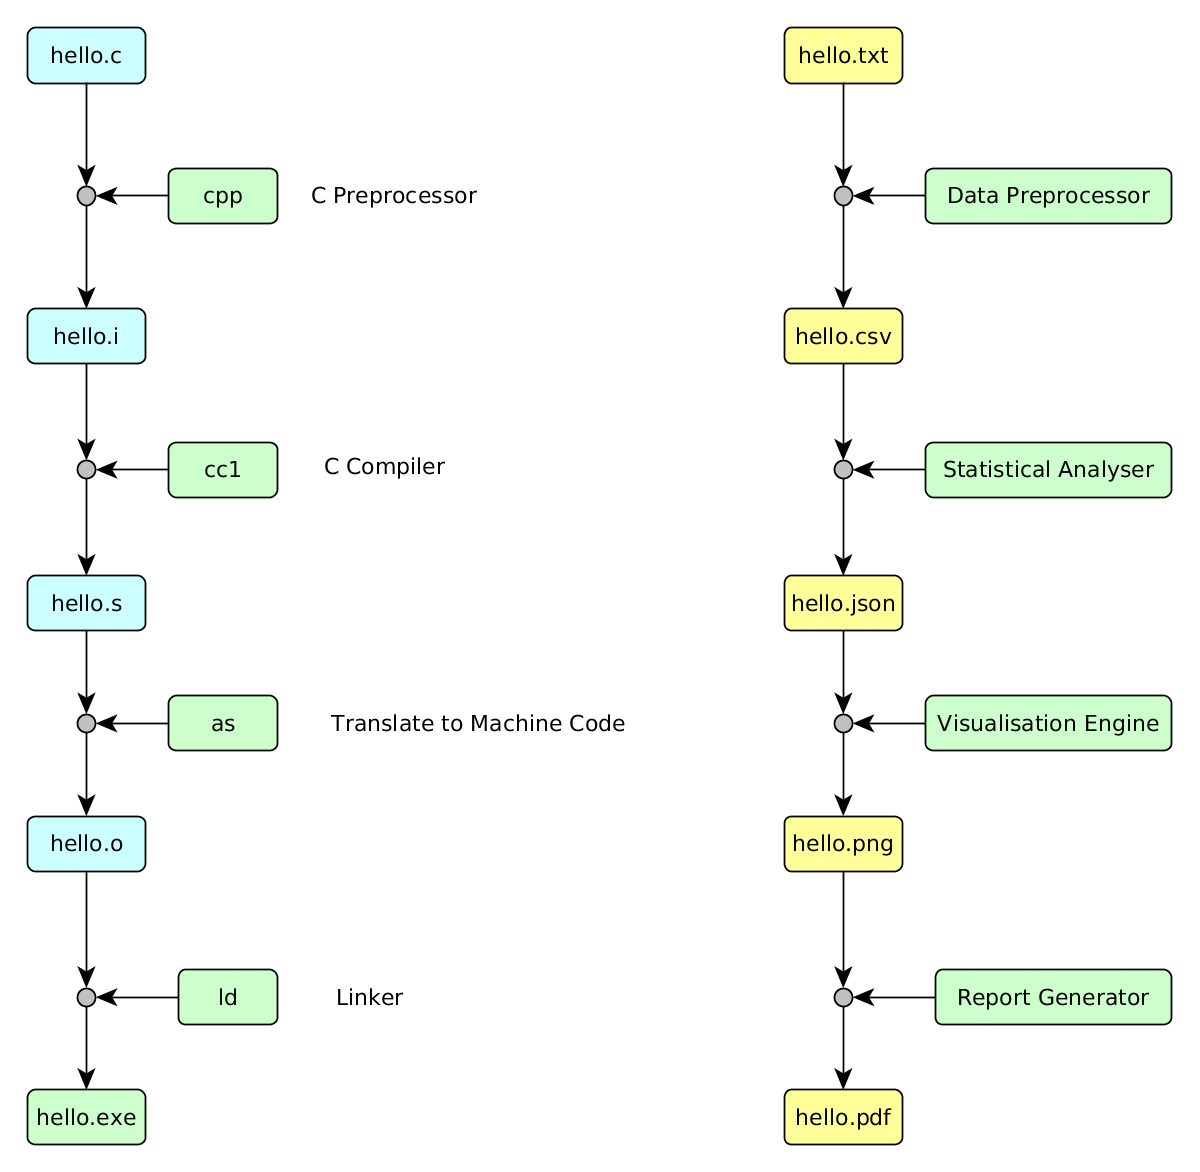
\includegraphics[width=\linewidth]{figs/dag/simple-chain.png}
\caption{Comparison of code build pipeline (left), and data processing pipeline (right). Source code artefacts are coloured blue, executable programs are coloured green, and datasets are coloured yellow. The distinction between source code, executable programs, and data is by convention (i.e. source code and executables are just specialised forms of data, but conventionally treated differently to datasets)}
\label{fig:simple-chain-cmp}
\end{figure}

On the left of \figref{fig:simple-chain-cmp} is an illustrative example of a code build process (the example is of compiling a program written in the C programming language; however, the programming language being used is immaterial here). The source code undergoes a series of compilations and linkage steps. At each stage an external program (part of the C compiler toolchain) transforms the code into an alternative form, typically with the goal of bringing high level code written by human software developers into a machine interpretable form. There are a range of build automation tools available, but conventionally one would use a Make\footnote{\url{https://en.wikipedia.org/wiki/Make_(software)}} script.

On the right of \figref{fig:simple-chain-cmp} is an example of a simple data processing pipeline. The data undergoes a series of extraction and analysis steps that transforms the data into an alternative form. At each stage an external program (e.g. bundled within a statistical analysis suite) transforms the data into an alternative form, typically with the goal of brining raw data (often machine collected) into a higher level form interpretable by human data analysts.

% even the non-apparent similarities...
There are similarities between the code build process and the data processing pipeline:
\begin{enumerate}
  \item While the build process operates on source code rather than datasets, source code is just a form of structured data. Furthermore, when operated on by a sufficiently sophisticated analysis, datasets themselves can act as source code. For example, if the dataset is processed by an inference engine, such as by converting facts in the dataset to statements in the Prolog logic programming language (which is Turing complete, i.e. capable of expressing arbitrarily complex programs), then the dataset functions as a form of source code.
  \item The final output of the build process is instructions interpretable by a machine. The final output of the data processing pipeline is information interpretable, or sometimes directly actionable, by a human.
\end{enumerate}

Note how these two tools may be unified to form a more complete picture of data provenance. Data processing pipelines track the flow of data acted upon by external executable programs (data preprocessor, statistical analyser, etc.). Reproducible build tools can be used to capture the full details of the build process used to arrive at these executable programs, including the recursive dependencies of the build such as the C preprocessor, C compiler, etc.\footnote{In practice, C compilers such as GCC are bootstrapped using an existing (possibly older) C compiler. However, in principle, all computations could be described using a small core of primitive concepts such as lambda calculus.} In theory, reproducible builds tools could also be used to construct complex data processing pipelines by tracking the user supplied data sources as dependencies of an ad-hoc build that is executed whenever a user runs an analysis on a data input. For example, the data processing pipeline on the right of \figref{fig:simple-chain-cmp} could in theory be represented as a reproducible build in the same way as software, the only limitations are that current reproducible build tools have not been designed to support this use case, thus the syntax for describing the build is awkward when one wants to perform quick ad-hoc analysis rather than reusable software.

% https://github.com/NixOS/nixpkgs/blob/master/pkgs/stdenv/linux/make-bootstrap-tools.nix
% https://nixos.org/nix/manual/
% https://stackoverflow.com/questions/9429491/how-are-gcc-g-bootstrapped
% https://github.com/NixOS/nix/issues/859 - Nix and IPFS #859

% (Image with DAG extension)

\subsubsection{Data Structures}

% Question should we use globally unique ids (GUIDs) rather than hashes? (e.g. if we need to distinguish between two datasets as being conceptually different despite having the same contents)

% We propose capturing the provenance information through the capture of triples (3-tuples):
This provenance information can be captured through triples (3-tuples):

$([Data\ input\ hash], Executable\ hash, [Data\ output\ hash])$

% \todo{compare to similar existing systems such as the Read, Write, State-Reset Provenance Model proposed by \cite{Bowers2006}}

Optionally, these can be extended to an \textit{n}-tuple to include auxiliary information such as timestamps. However, timestamps are not strictly necessary, as reconstruction of the execution graph allows sequencing the operations according to a partial ordering. Other auxiliary information one might want to capture includes system state that may help to with auditing if the execution is performed erroneously. However, for clarity of the provenance information, it will be assumed that the execution can be carried out correctly, for example by distributing the same computation out to independent computation nodes for validation\footnote{For example, in order to ensure smart-contracts are carried out correctly, the Ethereum blockchain runs the same calculation within a (highly optimised) virtual machine on every node on the network to obtain a consensus. This allows strong guarantees that the computation was performed correctly. However due to the high redundancy of having every node run the same operation, this method is only appropriate for small computations. ``A Next-Generation Smart Contract and Decentralized Application Platform'' \url{https://github.com/ethereum/wiki/wiki/White-Paper}. Accessed: \dt{2019-01-16}}.

% \todo{Explain a hash (for sport scientists). Explain the how this system would be exposed to the user (e.g. as a CLI similar to Git to help capture and query provenance)}

\subsubsection{Query of Provenance using Capture Log}

\begin{figure}[htbp]
\centering
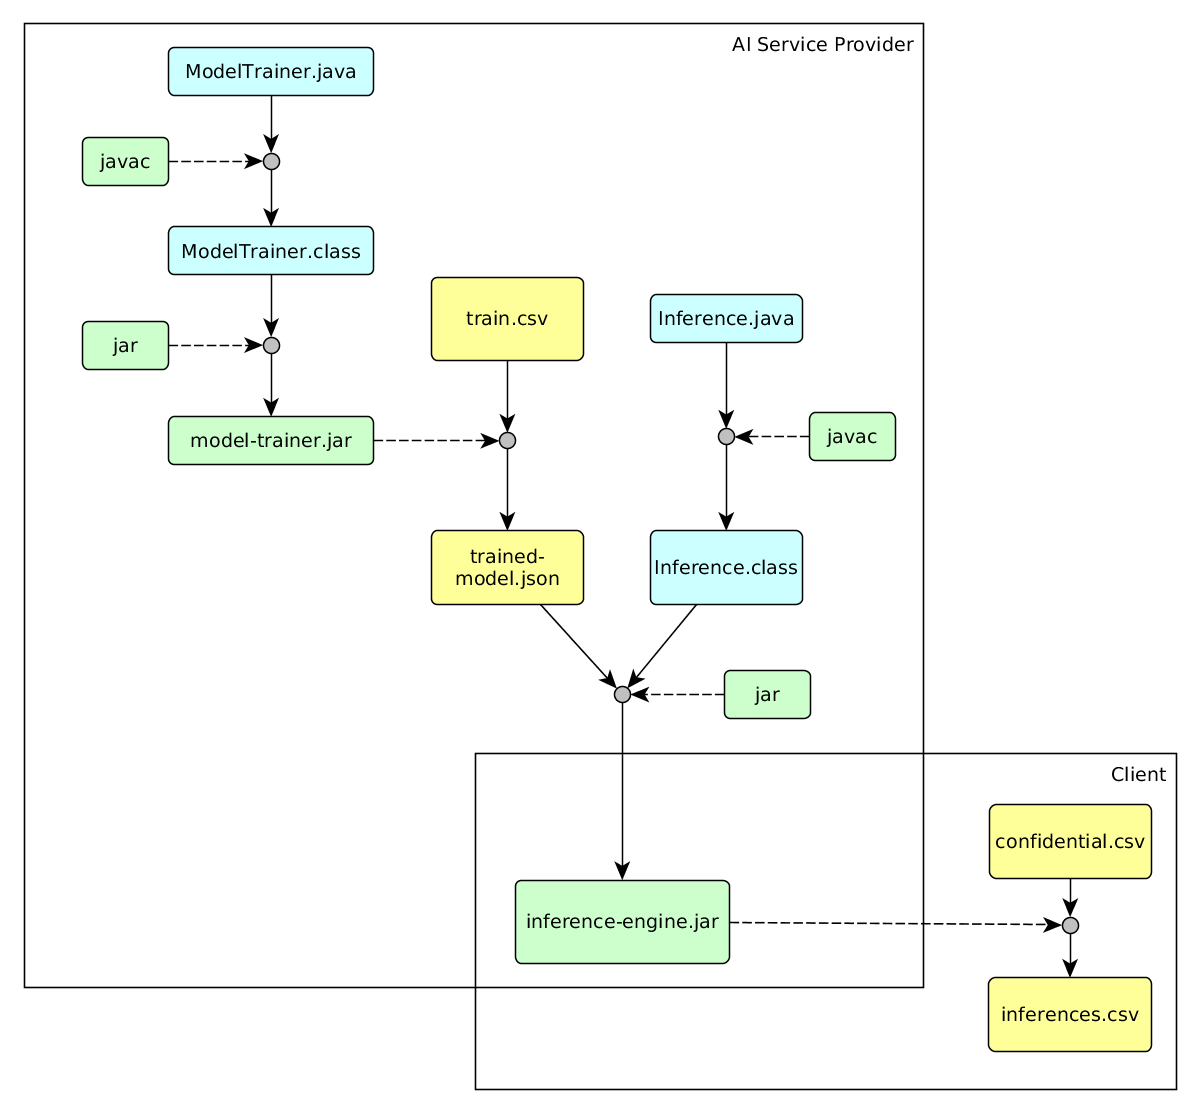
\includegraphics[width=\linewidth]{figs/dag/ml-build.png}
\caption{Sample Directed Acyclic Graph (DAG) for machine learning pipeline. Note the similarity of code artefacts (blue, green) and data artefacts (yellow). This suggests that the goal of achieving reproducible machine learning pipelines is equivalent to the problem of reproducible builds.}
\label{fig:ml-build}
\end{figure}

Capture of this information is enough to reconstruct the entire workflow graph and use it to query for provenance information. For example, given an output (such as ``output.csv''), and a full capture of the provenance triples, the provenance graph can be reconstructed to determine the inputs that contributed to ``output.csv''. If intermediate results are lost, they can be recomputed from the original inputs. An example workflow is provided in \figref{fig:ml-build}. Note that the ``Client'' in the diagram (e.g. analysts within the sport team), can trace the full provenance for confidential data (e.g. to re-identify individual players), whereas the ``AI Service Provider'' (e.g. external researchers working with sample de-identified data) can never see the confidential data (i.e. they only have a partial view of the system).

% \todo{simple example of reconstructing graph from a log of tuples}

\subsubsection{Relevance to Sport}

The value of having data structures to represent the computations performed in the form of a capture log, is that this allows queries to be run over the capture log to answer different data provenance questions. Specifically, in the context of sport, those data provenance queries would be questions of relevance to a sport performance analyst, such as \textit{``which years of game data were used to generate this analysis output?''}

Ultimately, the motivation for exploring computational pipelines and data provenance in this thesis, is to support the questions that sport coaches and practitioners would want to ask. This also includes surrounding questions that a sport performance analyst may need answered to verify the correctness of information. The next section of this thesis elaborates on what kinds of sport related questions could be expected, as well as the human-computer interface concerns that need to be considered to ensure that the results can be interpreted by sport practitioners.
